\section{Introduction}
\subsection{Background}

Thanks to the development of technology, self-driving cars and robots have become our daily routine, they have already changed and continue to change
the paradigms of transport and automation in various industries such as delivery, taxi, trucking and more.
The combination of the development of machine learning, robotics, mechatronics and input systems (cameras, lidars, radars, etc.) has become an important step towards
improving self-driving cars, robots and other systems, providing incredible opportunities and prospects in other areas.

Because of innovations in computer vision especially with using machine learning and deep learning as well as different types of sensors cars with autopilot and 
bots got a breakthrough in development.
Tesla with its autopilot for electric cars, Amazon with its research and implementation of autonomous delivery bots and other companies are great examples
of developing the industry.
These companies use different technologies like deep learning and different sensors (like lidars, cameras, gyroscopes, etc) for developing their algorithms.

The detection and labeling of environmental objects is an important factor for the operation of the perception system, which ensures the correct 
operation of autonomous cars and bots. To ensure safe and effective autonomous operation, detection and labeling processes must be configured accurately 
and reliably since these systems aim to simulate human perception and the ability to make their own decisions in unforeseen situations.

The perception and interpretation of complex environmental stimuli in real-time is made possible for autonomous vehicles and bots mainly through the use of 
detection and labeling algorithms. Using sensor data from cameras, lidar, radar and other detection tools, these algorithms simplify the search and identification 
of objects, obstacles and road infrastructure around the car. Also, accurate detection and labeling capabilities increase the vehicle's environmental awareness and 
allow proactive decisions to be made in dynamic driving conditions. Examples of how these algorithms work are the ability to distinguish between road signs,
road markups, as well as pedestrians and cyclists.

For the full functioning of a vehicle in autonomous driving scenarios, accurate identification and labeling of possible hazards is crucial to reduce risks 
and ensure the prevention of various types of accidents. Active collision avoidance techniques such as emergency braking or maneuverable steering are made 
possible by fast and well-established detection and marking systems that recognize and classify objects and obstacles in the path of an autonomous vehicle. 
Reliable detection algorithms also have the ability to predict unforeseen situations to some extent, such as unexpected pedestrian crossings or strange vehicle 
behavior, and respond to them with the slightest delay, increasing overall road safety and thus reducing the risk of accidents.

In addition to recognizing objects, labeling algorithms help with semantic understanding and contextual interpretation of the environment. 
These methods allow a vehicle to distinguish between different types of objects (for example, vehicles, pedestrians and bicycles) and draw conclusions about 
their possible behavior by providing semantic labels and attributes to identified elements and entities. Making rational navigation decisions, such as giving 
way to pedestrians at pedestrian crossings or reconciling complex traffic scenarios with numerous parallel interacting road users, depends on this semantic 
understanding.

Reliability, as well as the ability to adapt to rapidly changing circumstances, are also necessary for detection and marking systems to cope with their 
inherent unpredictability and variety of situations in the real world. Autonomous vehicles and robots face a number of obstacles and circumstances that 
affect the accuracy of detection and labeling algorithms, such as changing lighting conditions, interference or noise in sensors. Therefore, in order to improve 
the performance of these algorithms and generalization capabilities in various work situations, continuous optimization and refinement using machine learning and 
methodologies based on the data obtained is crucial.

Summing up, we can say that the perception systems in autonomous cars and bots mostly rely on detection and labeling systems as fundamental building blocks that 
allow them to perceive, see, understand and overcome difficult situations on their own. In order to ensure safer and more efficient autonomous operation, 
and in addition to increase awareness of the autonomous transport environment, as well as reduce risks and facilitate smooth interaction with it, detection and 
labeling algorithms must be sufficiently accurate, reliable and flexible.

\subsection{Context}
In March \- April of 2023 I was a participant in Joint Advanced Student School (JASS) by JetBrains. 
There we developed a smart city prototype using the Duckietown project. I have noticed that Duckiebots \- robots that imitate self-driving cars in a smart city behave 
differently with different lightning. For example, we always kept curtains closed, but if the wind flow opened them the bot started driving unpredictably.

After a small investigation, I've discovered, that the current algorithm that is run on Duckiebots is based on segmenting pixels by colors. This approach is good when 
light conditions are constant, but each time they change (new room with different lightning or changing time in a room with opened curtains) 
the bot needs recalibration. Also important to mention that each Duckiebot has LED lights that can be almost any color which can lead to wrong detection.

\begin{figure}[htbp]
    \centering
    \subfloat[Raw image of the road with the first light condition]{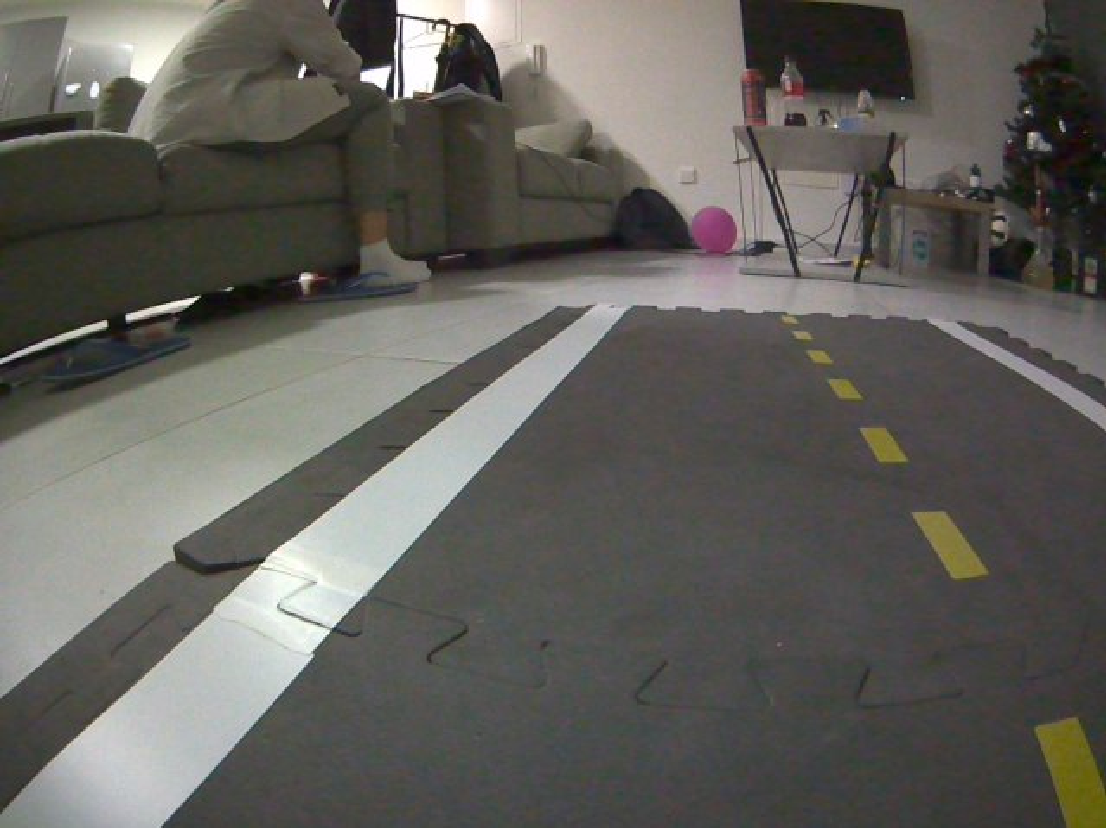
\includegraphics[scale=0.1]{src/Introduction/assets/old_masks2.png}}
    \subfloat[Mask of the road with the first light condition]{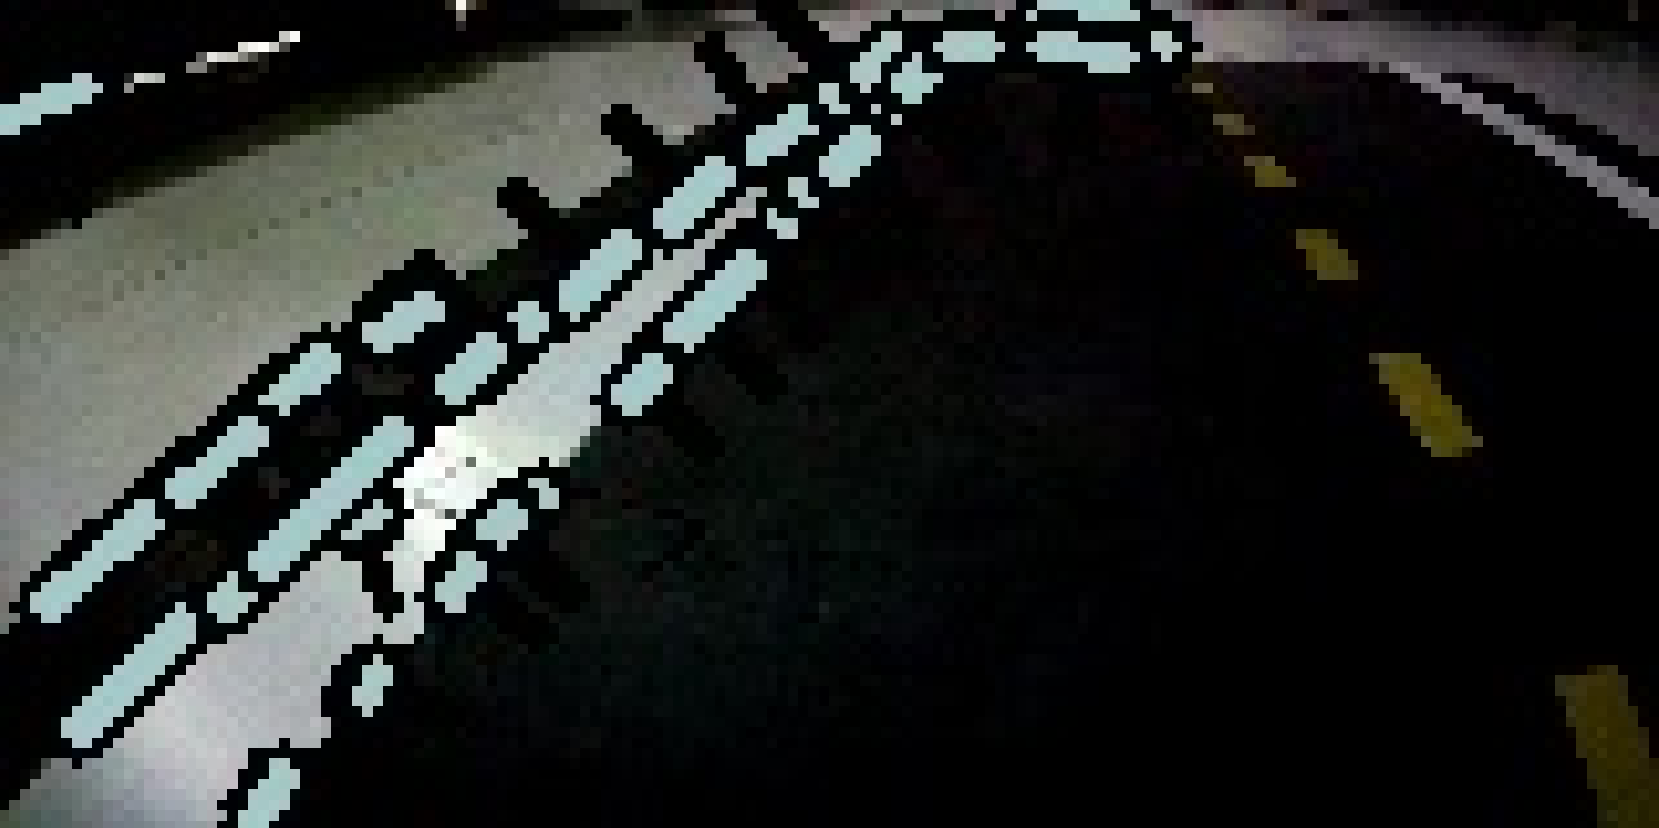
\includegraphics[scale=0.1]{src/Introduction/assets/old_masks1.png}}
    \\
    \subfloat[Raw image of the road with the second light condition]{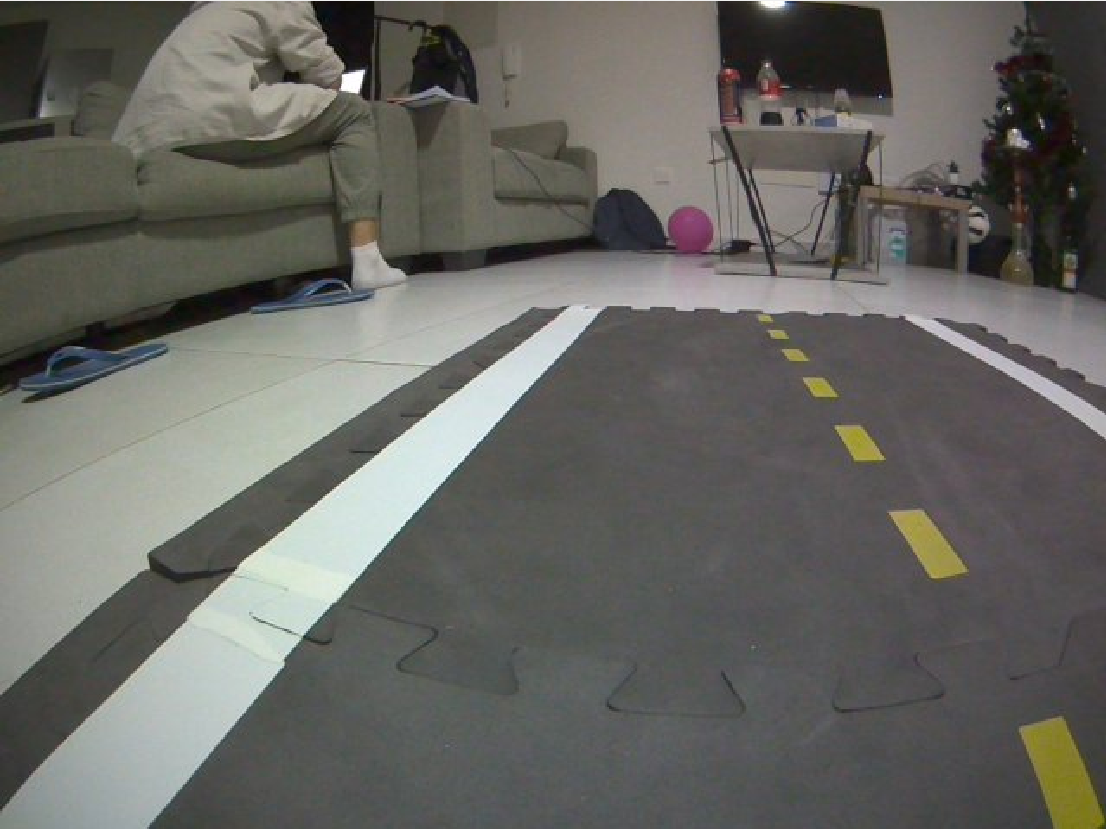
\includegraphics[scale=0.1]{src/Introduction/assets/old_masks3.png}}
    \subfloat[Mask of the road with the second light condition]{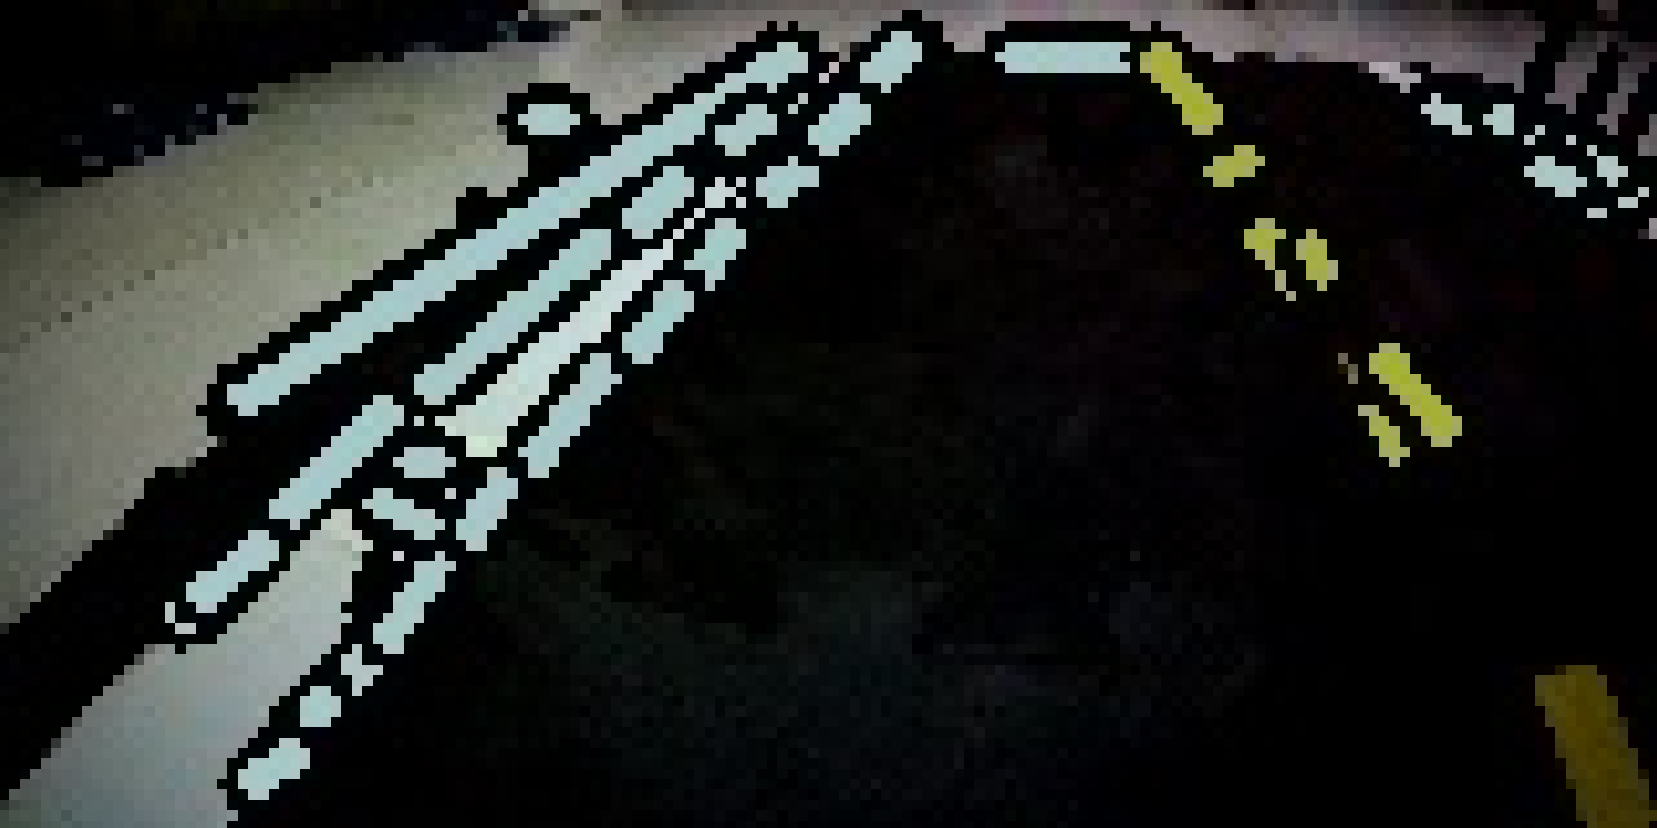
\includegraphics[scale=0.1]{src/Introduction/assets/old_masks4.png}}
    \caption{Old algorithm segmentation with different light conditions}\label{fig:old_masks}
\end{figure}
\subsection{Applicability of Findings to the Commercial World}

So after this observation, the idea of developing a light-insensitive road markup detection algorithm came to my mind. 
I wanted to create an algorithm based on the deep learning (DL) approach, so it would be easy to scale (in terms of developing a new neural network), 
light-insensitive, but at the same time light in computational terms.


\subsection{Bot specification}
The idea of using the DL approach came to me as soon as 
I've discovered that Duckiebots can be powered by Jetson Nano by Nvidia.

\begin{table}[h]
    \centering 
    \begin{tabular}{|c|c|}
        \hline
        AI Performance & 472 GFLOPs \\ \hline
        GPU & 128-core NVIDIA Maxwell™ GPU \\ 	\hline
        CPU & Quad-Core ARM® Cortex®-A57 MPCore  \\ \hline
        Memory & 4GB 64-bit LPDDR4 Memory \\ \hline
        Storage & Micro SD \\\hline
    \end{tabular} % Конец определения столбцов таблицы
    \caption{Jetson nano specs} % Подпись к таблице
    \label{tab:example} % Метка для ссылки на таблицу
\end{table} % Конец окружения таблицы

4GB of RAM and 128 CUDA cores are more than enough for a lightweight 
convolutional neural network (CNN)